\documentclass[12pt]{report}
\usepackage[brazil]{babel}
\usepackage[utf8]{inputenc}
\usepackage{minted}
\usepackage{tabularx}
\usepackage{booktabs}
\usepackage{graphicx}
\usepackage{float}

\sloppy
\renewcommand{\arraystretch}{1.15}
\title{Projeto PIC10F202}
\author{Pedro Faria Fernandes, Vinícios Bidin, Bruno Oliveira}
\date{01 de junho de 2023}

\begin{document}
	\maketitle
	\section*{Questão 1}
		Este algoritmo consiste em um somatório de 9 até 0, pois tem-se um laço de repetição com o seguinte critério de parada: o valor do registrador \texttt{mem[0$\times$08]}
		após o decremento de 1 do valor deste, na \textit{label} `loop', precisa ser 0. Neste caso, o programa irá pular para a \textit{label} `break', onde irá pular para o final do programa.

		O literal carregado para o registrador `w', na primeira linha da \textit{label} `main', é 10. Porém, como no critério de parada, antes de ser armazenado o valor da soma no registrador `w', é decrementado em um o valor de `w'. Por conta disso, trata-se de um somatório do valor de $w - 1$ até 0: $\sum\limits_{i=w-1}^{1}i$.

		A seguir, tem-se o equivalente ao código feito na linguagem de programação C:\@
	\begin{minted}{c}
	int main(void) {
		int w, f;
		f = w;
		w = 0;

		while (--f) {
			w += f;
		}

		f = w;
		return 0;
	}
	\end{minted}
	\clearpage
	\section*{Questão 2}
		\begin{verbatim}
main:
    ; $w é o registrador W do PIC10F202
    ; Mapeamento entre endereços do File Register e variáveis: 
    ; 0x08 = x
    ; 0x09 = y
    ; 0x0A = z
    ; 0x0B = q

    MOVLW 4 ; $w = 4
    MOVWF 0x08 ; x = $w

    MOVLW 7 ; $w = 7
    MOVWF 0x09 ; y = $w
loop:
    MOVF 0x08, 0 ; $w = x
    ADDWF 0x09, 0 ; $w = $w + y
    MOVWF 0x0A ; z = $w -> z = x + y
		
    MOVF 0x08, 0 ; $w = x
    ANDWF 0x09, 0 ; $w = $w & y
    MOVWF 0x0B ; q = $w -> q = x & y
		
    MOVF 0x0A, 0 ; $w = z
    SUBWF 0x0B, 0 ; $w = $w - q
    BTFSC STATUS, 2 ; Sw $w for zero, pula a próxima instrução. 
    GOTO end ; equivalente a 'break'
		
    DECFSZ 0x08, 1 ; x = x - 1 e se o resultado for zero,
    ; pula a próxima instrução.
    GOTO loop
end:
    END ; return 0
		\end{verbatim}
	\section*{Questão 3}
		\begin{figure}[H]
			\centering
			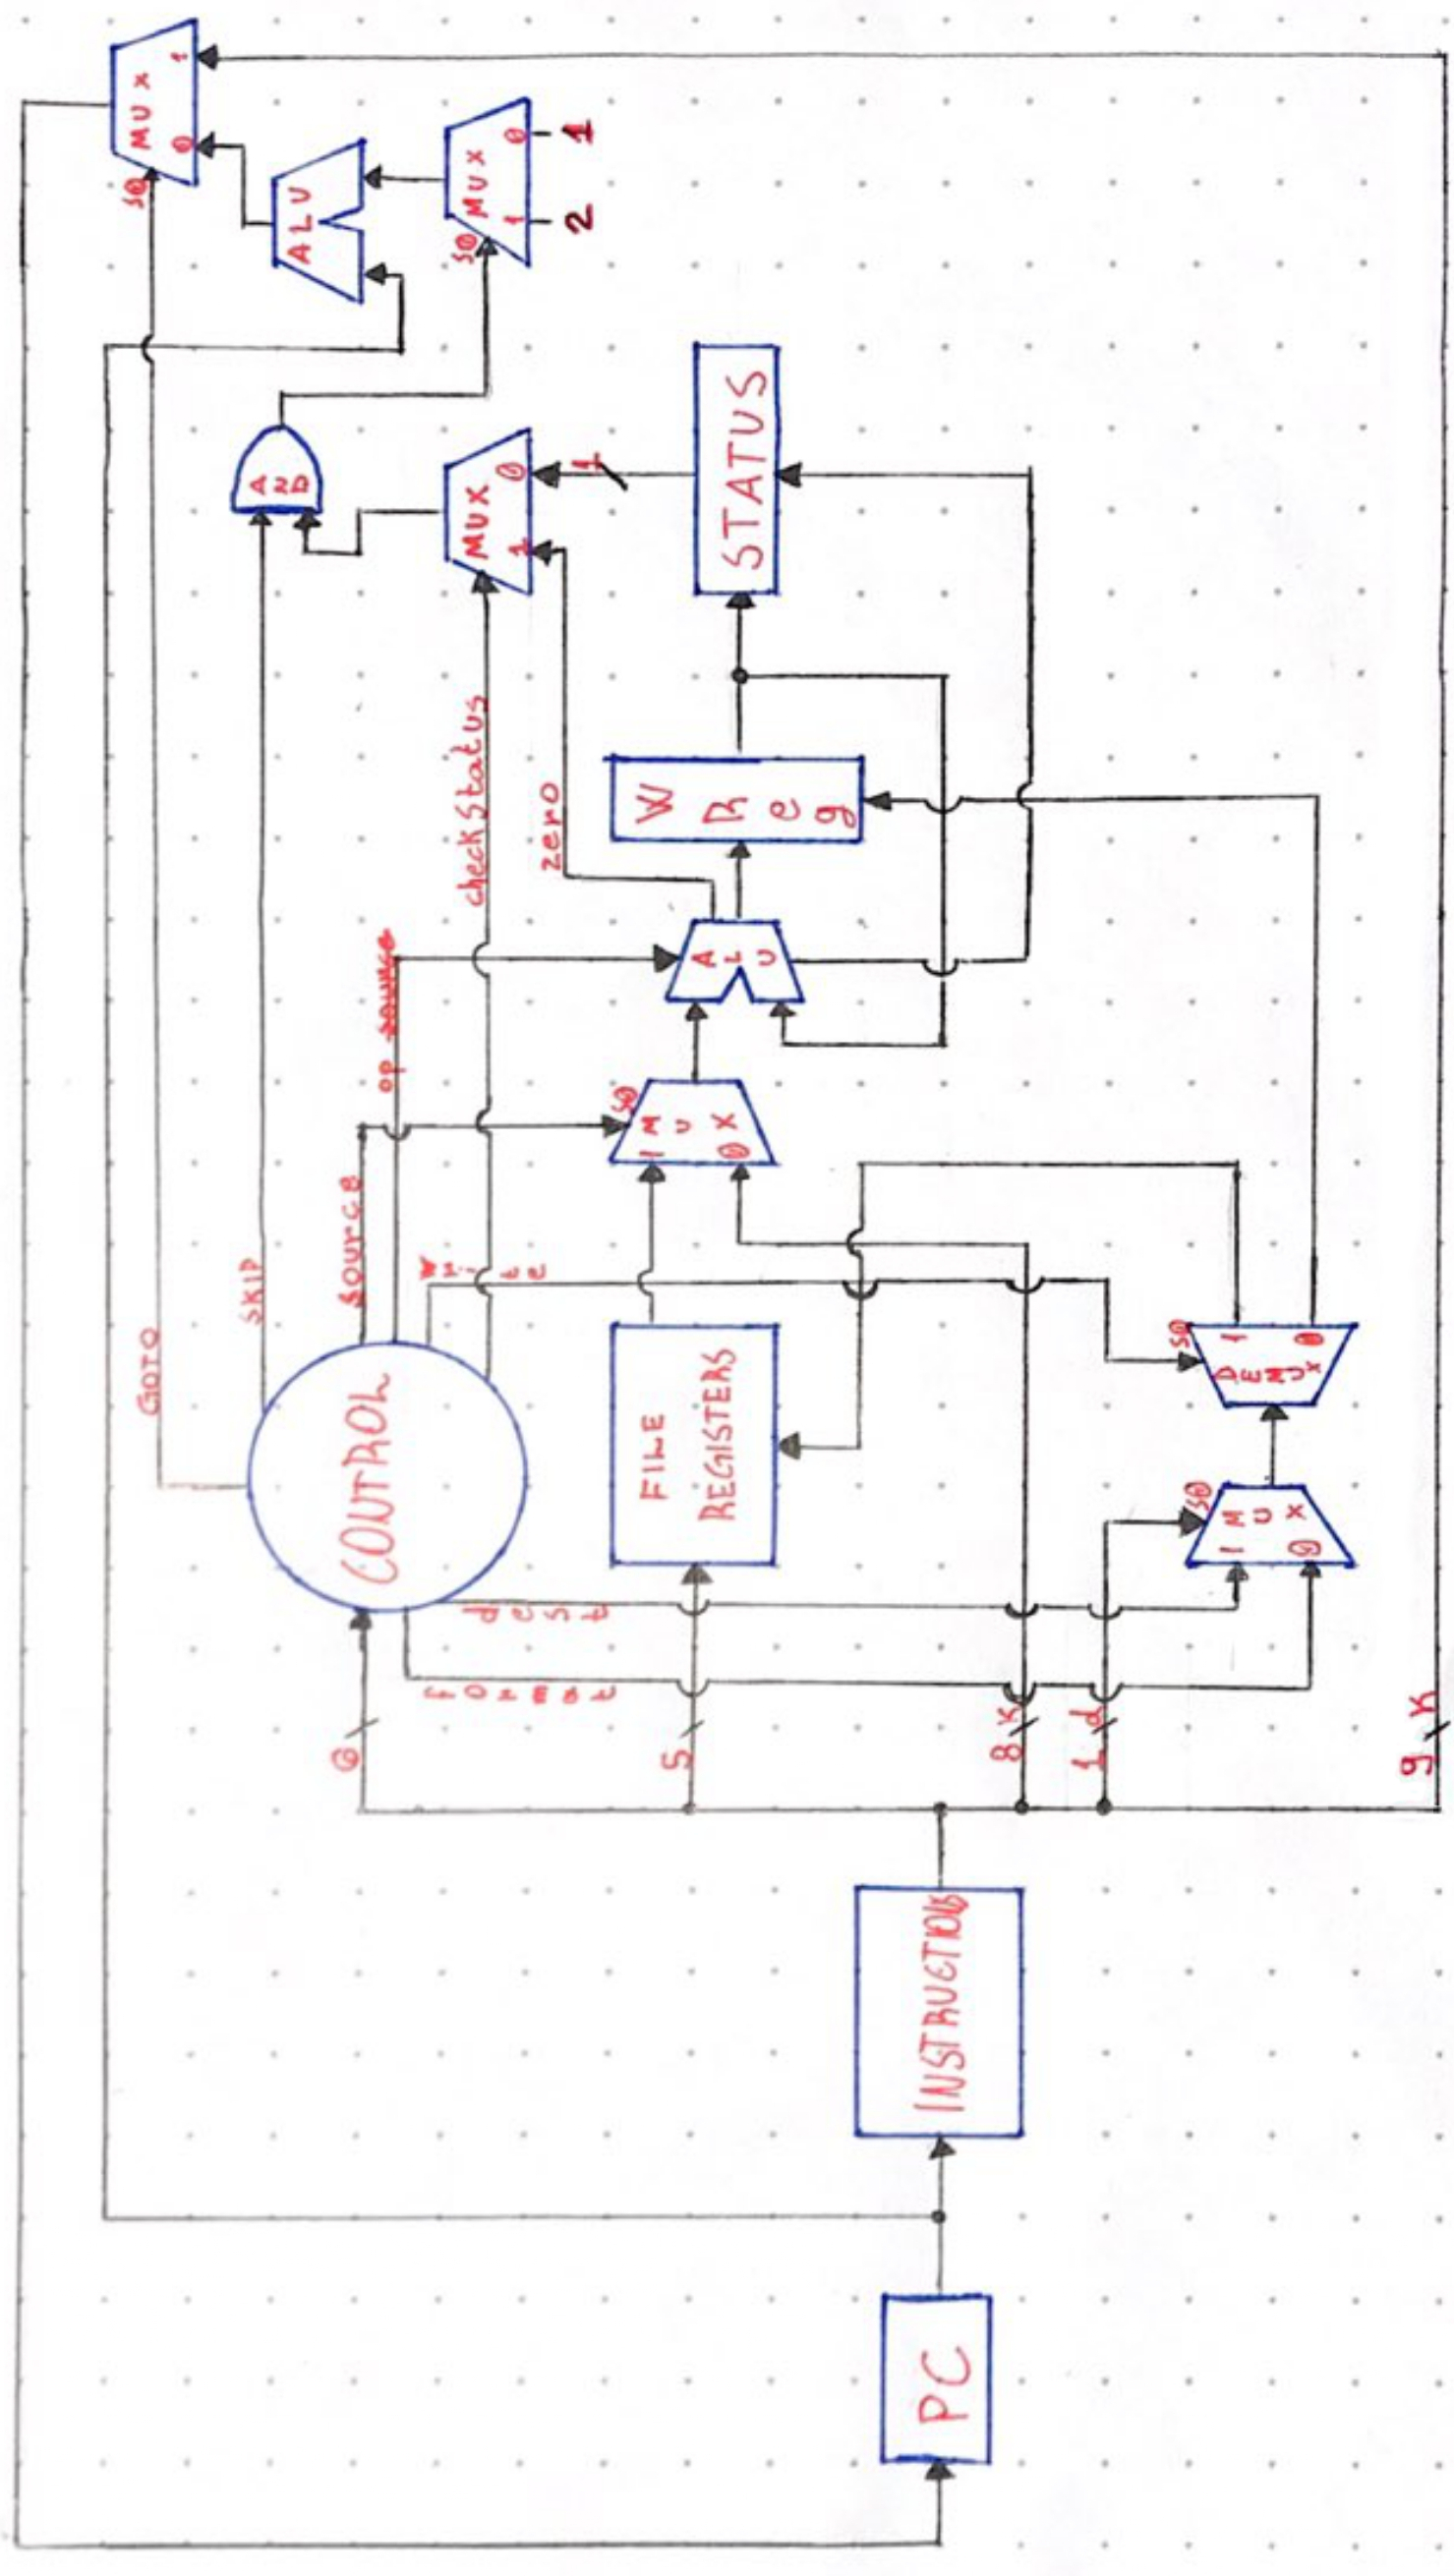
\includegraphics{datapath.jpg}
		\end{figure}
	\clearpage
	\section*{Questão 4}
		\begin{table}[ht]
			\centering
			\caption{\textbf{Sinais de controle}}
			\begin{tabular}{ccccccccc}
				\toprule
				\textbf{Instr} & \textbf{w} & \textbf{frmt} & \textbf{dest} & \textbf{op} & \textbf{src} & \textbf{skip} & \textbf{goto} & \textbf{chkStatus} \\
				\midrule
				MOVLW & 1 & 0 & 0 & MOV & 1 & 0 & 0 & x \\
				MOVWF & 1 & 1 & x & MOV & 0 & 0 & 0 & x \\
				MOVF & 1 & 1 & x & MOV & 0 & 0 & 0 & x \\
				ADDWF & 1 & 1 & x & ADD & 0 & 0 & 0 & x \\
				ANDWF & 1 & 1 & x & AND & 0 & 0 & 0 & x \\
				SUBWF & 1 & 1 & x & SUB & 0 & 0 & 0 & x \\
				BTFSC & 0 & x & x & x & x & 1 & 0 & 1 \\
				GOTO & 0 & x & x & x & x & x & 1 & x \\
				DECFSZ & 1 & 1 & x & x & 0 & 1 & 0 & 0 \\
				\bottomrule
			\end{tabular}\label{tab:Sinais de controle}
			\begin{tabularx}{\textwidth}{l X}
				\textbf{Nota:} & Abreviações utilizadas na tabela --- \textit{w}: write, \textit{frmt}: format, \textit{src}: source, \textit{chkStatus}: checkStatus.
			\end{tabularx}
		\end{table}
\end{document}
